\section{STFT of kepler data}

Here we try use Matlab STFT spectrogram function to look for any prevalent frequency change over the observation time. 
We try to find a windows function that will give us more frequency resolution, the data is already very noisy and normal rectangular window will give a lot of articulates that will pollute the spectral plot. We go with blackman. The windows size is a trade-of between time resolution and frequency resolution, we go for something in between and as the number of samples is 4654 we go for 128.    
\\
The spectrogram plot is shown in figure \ref{fig:STFT}. It is very difficult to see any change. This is due to very low data count and slow / very small changes, coupled with a lot of noise. 

\begin{figure}[h]
  \centering
  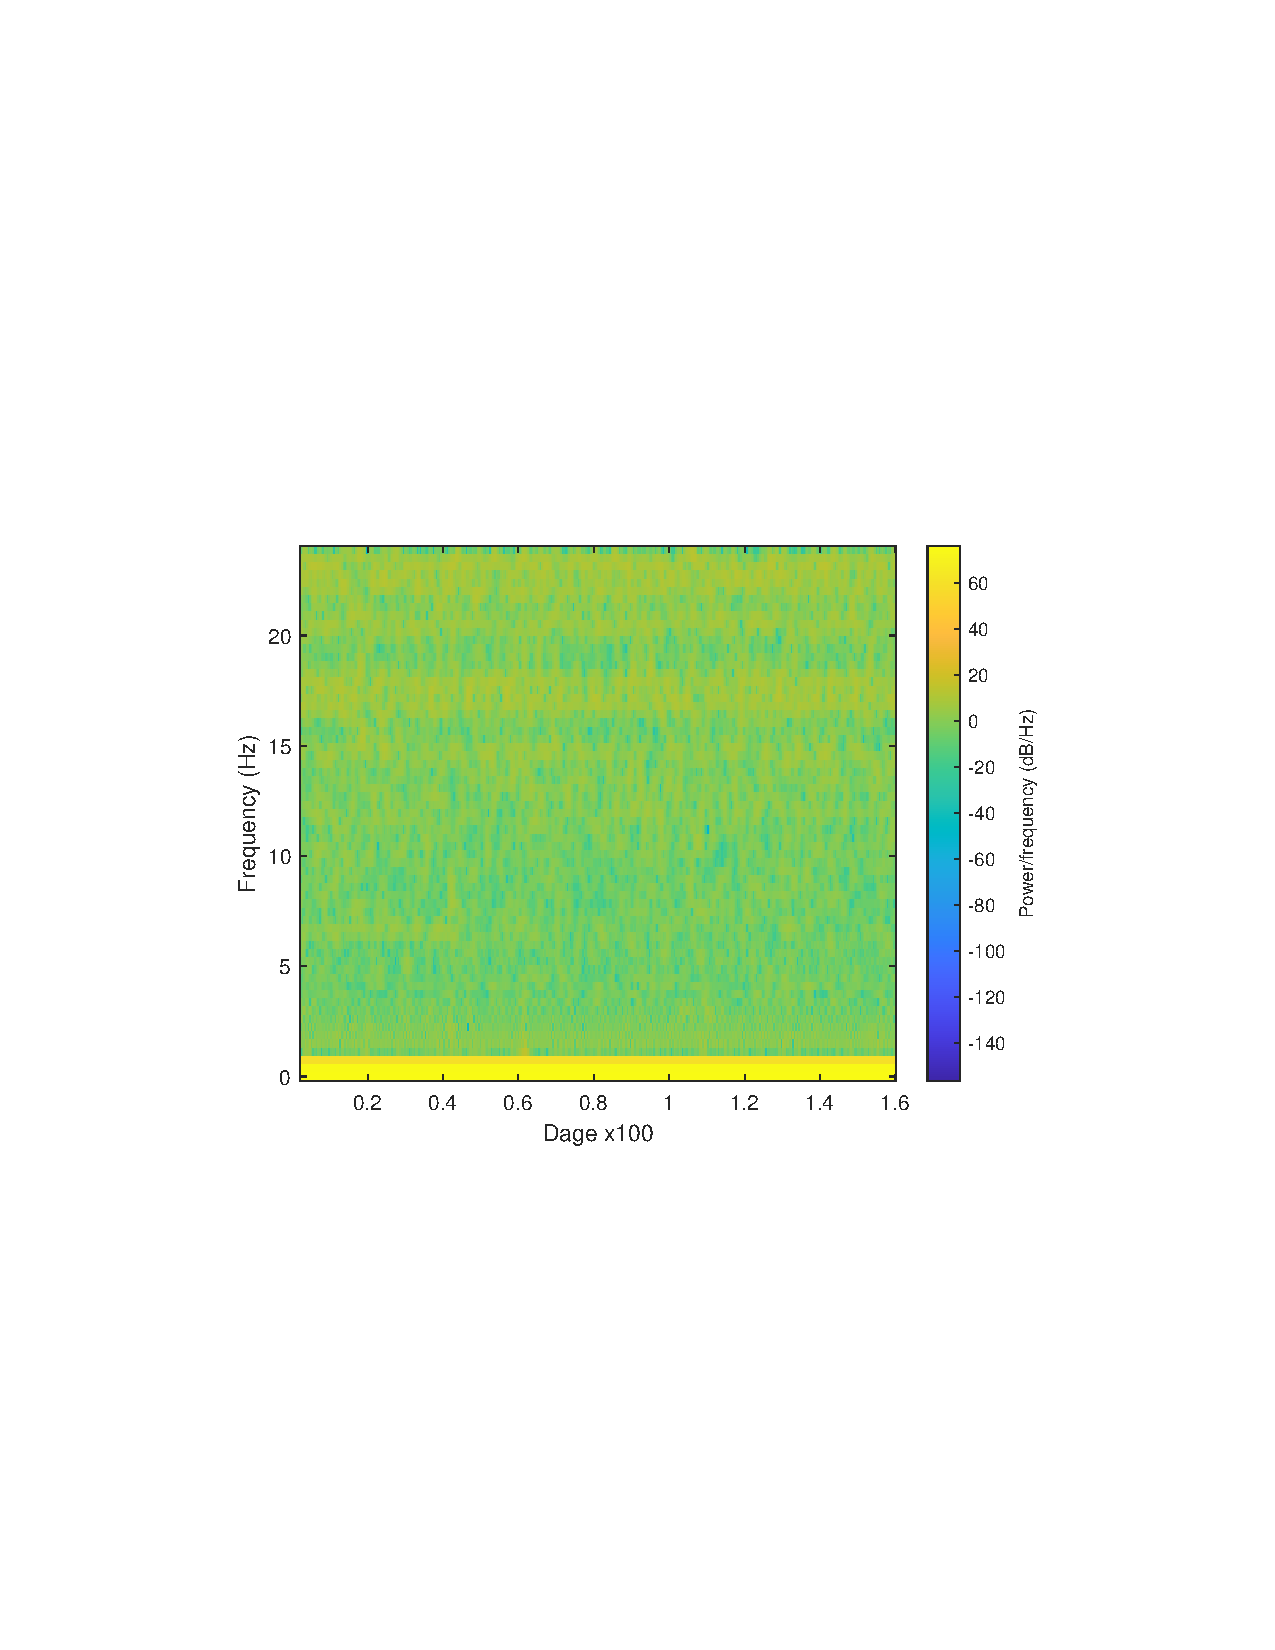
\includegraphics[width=\textwidth]{matlabstuff/STFT.pdf}
  \caption{STFT spectrogram of the kepler data}%
  \label{fig:STFT}
\end{figure}

\begin{figure}[h]
  \centering
  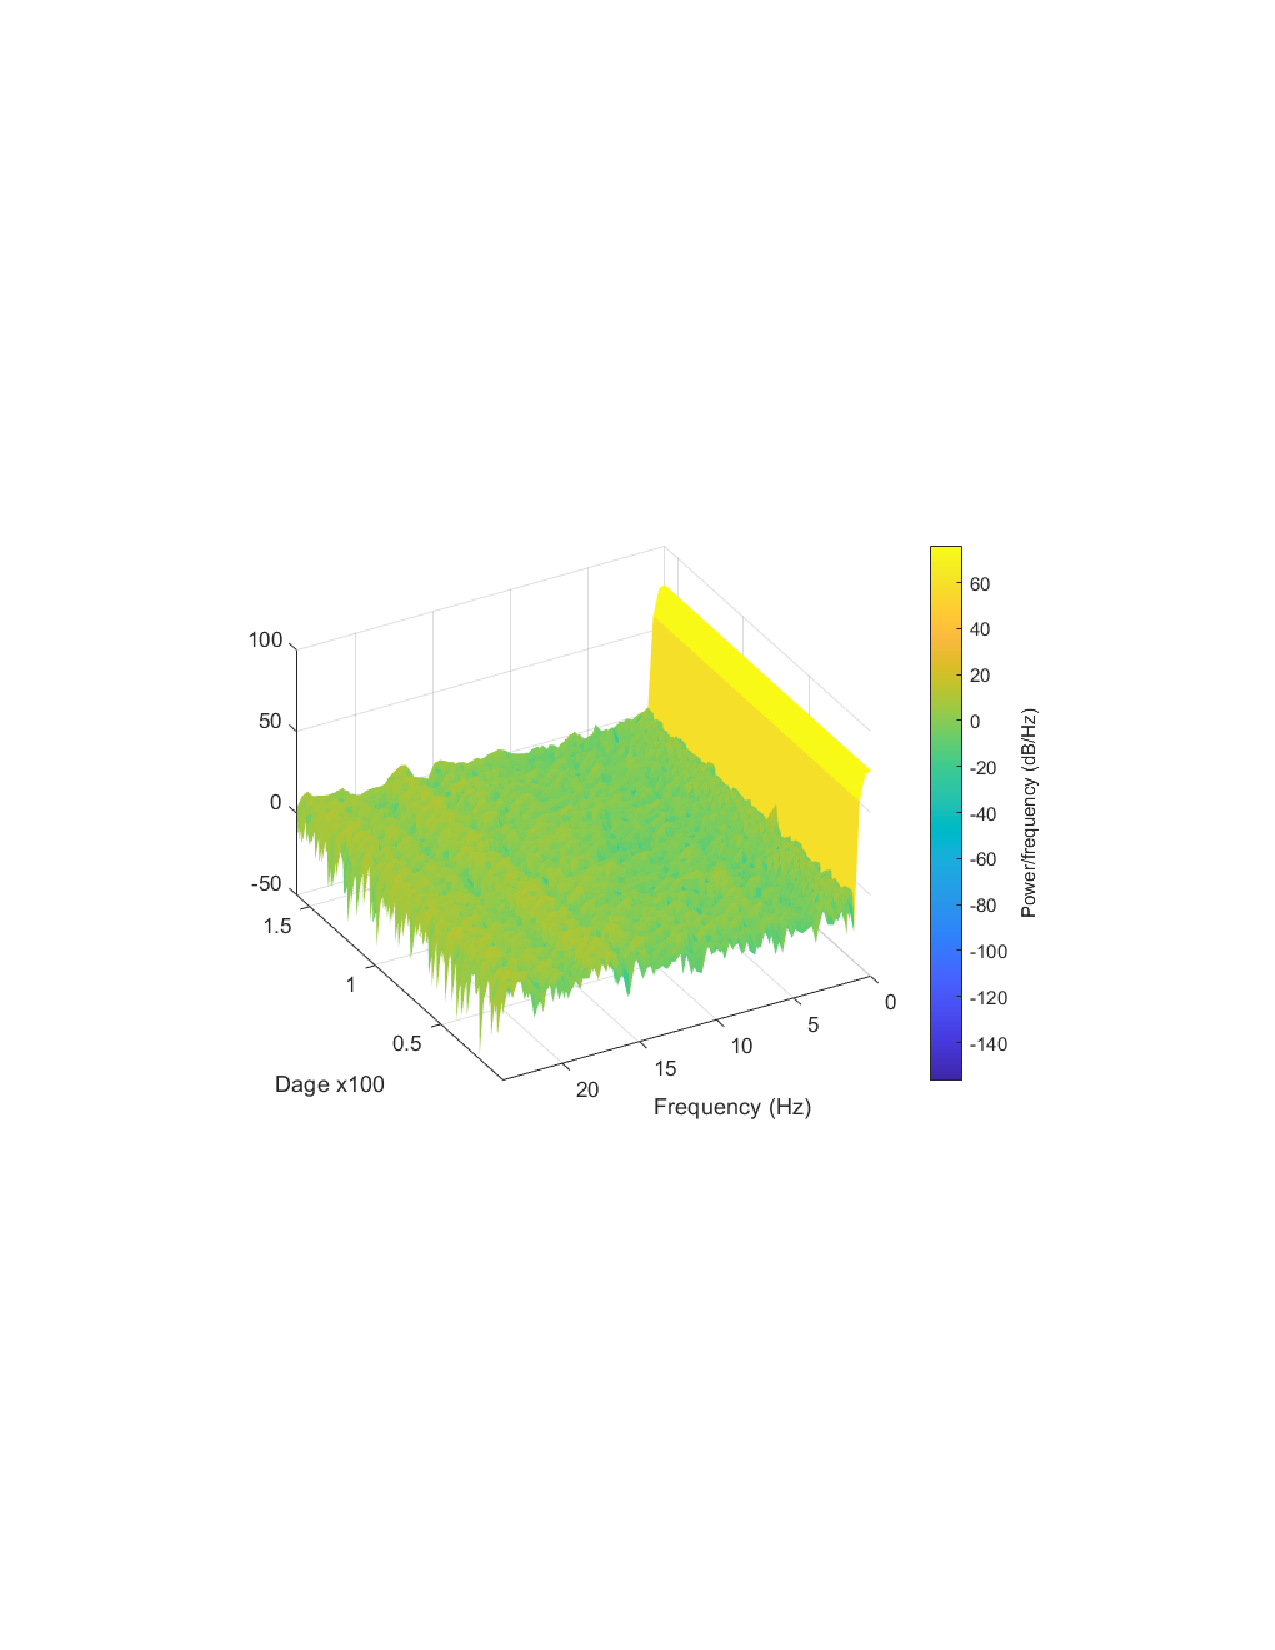
\includegraphics[width=\textwidth]{matlabstuff/mesh_stft.pdf}
  \caption{STFT spectrogram of the kepler data}%
  \label{fig:STFT}
\end{figure}
